% ==============================================================================
% THBKG Research Poster - A0 Portrait - beamerposter
% QMUL Brand Colour Scheme
% ==============================================================================
\documentclass[final,t]{beamer}
\usepackage[size=a0,scale=1.3,orientation=portrait]{beamerposter}

\setbeamertemplate{navigation symbols}{}

% Packages
\usepackage{graphicx}
\usepackage{amsmath,amssymb}
\usepackage{booktabs}
\usepackage{tikz}
\usetikzlibrary{shapes.geometric, arrows.meta, positioning}
\usepackage{tcolorbox}
\tcbuselibrary{skins}
\usepackage[T1]{fontenc}
\usepackage{ragged2e}
\usepackage{subcaption}

% ==============================================================================
% QMUL BRAND COLOURS
% ==============================================================================
\definecolor{qmulblue}{RGB}{0,32,92}        % #00205C
\definecolor{qmulgold}{RGB}{205,168,44}      % #CDA82C
\definecolor{qmulbluelight}{RGB}{0,71,186}   % #0047BA
\definecolor{blockbg}{RGB}{245,248,252}
\definecolor{accentgreen}{RGB}{46,139,87}
\definecolor{accentred}{RGB}{178,34,34}

% Beamer colour assignments
\setbeamercolor{block title}{bg=qmulblue,fg=white}
\setbeamercolor{block body}{bg=blockbg,fg=black}
\setbeamercolor{block alerted title}{bg=qmulgold,fg=qmulblue}
\setbeamercolor{block alerted body}{bg=blockbg,fg=black}

% Font sizes
\setbeamerfont{block title}{size=\LARGE,series=\bfseries}
\setbeamerfont{block body}{size=\normalsize}

\setbeamertemplate{headline}{}
\setbeamertemplate{footline}{}
\setbeamersize{text margin left=20mm, text margin right=20mm}

% Custom command
\newcommand{\eahgt}{\textsc{EA-HGT}}

\begin{document}
\begin{frame}[t]

% ==============================================================================
% HEADER
% ==============================================================================
\begin{tikzpicture}[remember picture, overlay]
  \fill[qmulblue] ([yshift=2mm]current page.north west) rectangle
    ([yshift=-14cm]current page.north east);
  \fill[qmulgold] ([yshift=-14cm]current page.north west) rectangle
    ([yshift=-14.5cm]current page.north east);
\end{tikzpicture}

\vspace{-1.2cm}

\begin{columns}[T]
  \begin{column}{.86\linewidth}
    \vspace{0.5cm}
    \begin{center}
      {\color{white}\VeryHuge\bfseries
        THBKG: A Temporal Heterogeneous Biomedical
        Knowledge Graph for Clinical Trial
        Advancement Prediction}\\[0.8cm]
      {\color{white}\Large\bfseries
        Siu Pui Chung\textsuperscript{1,3}\quad
        Claudia Cabrera\textsuperscript{2,*}\quad
        Mani Mudaliar\textsuperscript{3}\quad
        Arkaitz Zubiaga\textsuperscript{1,*}}\\[0.4cm]
      {\color{white}\normalsize
        \textsuperscript{1}EECS, Queen Mary University of London\quad
        \textsuperscript{2}William Harvey Research Institute, QMUL\quad
        \textsuperscript{3}Recursion Pharmaceuticals}
    \end{center}
  \end{column}
  % \begin{column}{.10\linewidth}
  %   \begin{center}\vspace{0.8cm}
  %     % REPLACE with: \includegraphics[width=0.85\linewidth]{logos/event_logo.png}
  %     \begin{tikzpicture}
  %       \node[draw=white, line width=1.5pt, rounded corners=5pt,
  %             minimum width=4cm, minimum height=4cm,
  %             text=white, font=\large\bfseries, align=center] {Event\\Logo};
  %     \end{tikzpicture}
  %   \end{center}
  % \end{column}
\end{columns}

\vspace{0.4cm}

% ==============================================================================
% KEY MESSAGE BAR
% ==============================================================================
\begin{tcolorbox}[
  colback=qmulgold!12, colframe=qmulgold, boxrule=2.5pt, arc=5pt,
  left=10mm, right=10mm, top=5mm, bottom=5mm
]
\centering
{\Large\bfseries\color{qmulblue}
We construct the first temporally-indexed biomedical knowledge graph that enables quasi-prospective clinical advancement prediction, outperforming the state-of-the-art ridge regression baseline under decision-aligned evaluation.}
\end{tcolorbox}

\vspace{0.15cm}

% ==============================================================================
% MAIN CONTENT
% ==============================================================================
\begin{columns}[T]

% ======== LEFT COLUMN =========================================================
\begin{column}{.47\linewidth}

\begin{block}{Motivation}
{\normalsize
Ranking target--disease programmes by likelihood of Phase~II$\rightarrow$III advancement can direct drug development resources toward better-supported bets.

\vspace{0.15cm}

\begin{itemize}
  \item $\sim$90\% of candidates fail; wrong target selection drives 40--50\% of Phase~II efficacy failures
  \item \textbf{Temporal inflation}: calendar-split evaluation flatters models because successful targets accumulate evidence faster, so models learn to recognise advancement \emph{already happened}
  \item \textbf{Quasi-prospective evaluation} (Czech et al., 2024) removes this: each pair scored using only pre-decision evidence, revealing \textbf{75.4\% have zero direct evidence}
  \item Indirect paths compensate (Falaguera et al., 2025): 44\% indirect genetic support vs.\ 23\% direct
\end{itemize}
}
\end{block}

\vspace{0.15cm}

\begin{block}{THBKG Construction}
{\normalsize
\begin{itemize}
  \item \textbf{Pipeline}: Open Targets 23.06 $\rightarrow$ temporally-indexed heterogeneous graph reconstructing the evidence landscape at any historical decision point
  \item \textbf{5 node types} (target, disease, molecule, pathway, GO term), \textbf{19 edge types} (16 temporal, 3 static)
  \item \textbf{Task}: predict Phase~II$\rightarrow$III advancement; each pair scored with pre-decision evidence only ($t_{ij} < y$)
\end{itemize}
}

\vspace{0.15cm}

\begin{center}
  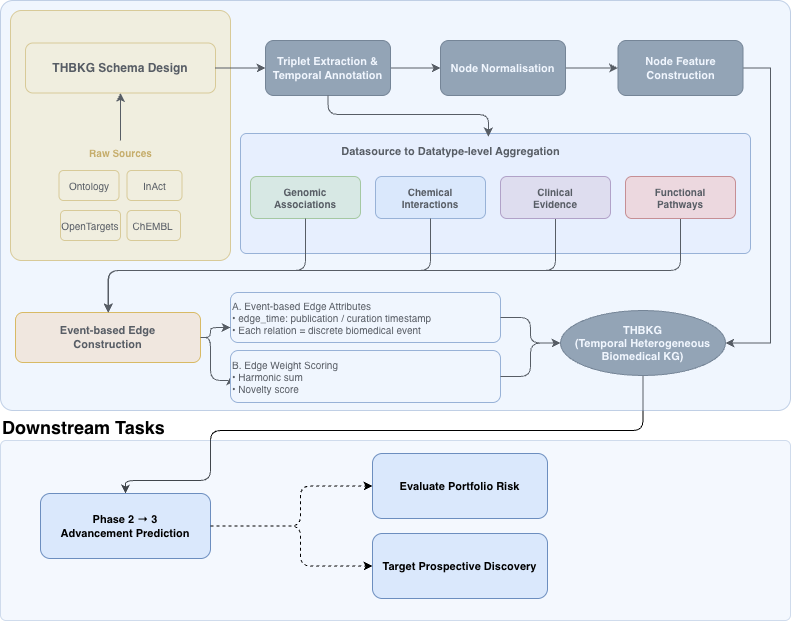
\includegraphics[width=0.85\linewidth]{figures/THBKG_pipeline_schema.drawio.png}
\end{center}
\end{block}

\vspace{0.15cm}

\begin{block}{Graph Overview}
{\normalsize
\begin{itemize}
  \item \textbf{5 node types}, \textbf{19 relation types} (16 temporal, 3 static)
  \item The graph grows substantially denser between 2010--2020; models on the full graph see richer neighbourhoods than existed at earlier decision points, motivating quasi-prospective masking
\end{itemize}
}

\vspace{0.15cm}

\noindent\begin{minipage}[c]{0.48\linewidth}
  \centering
  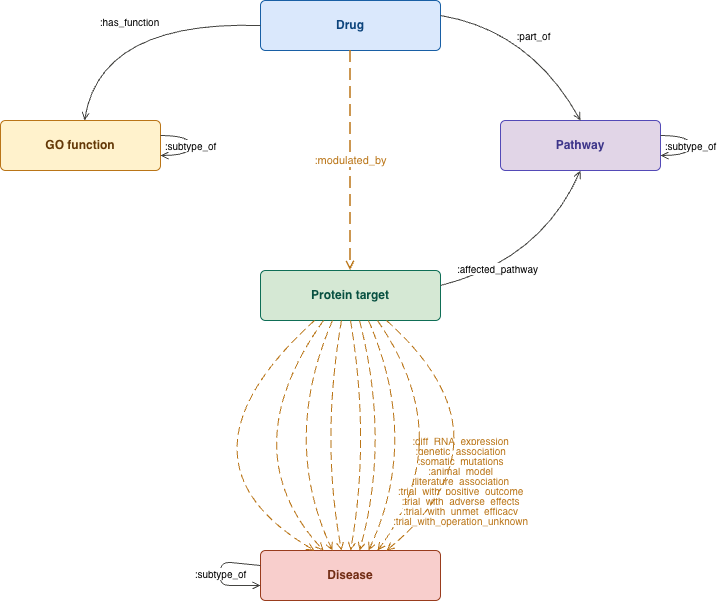
\includegraphics[width=\linewidth,height=14cm,keepaspectratio]{figures/THBKG_schema.drawio.png}
\end{minipage}%
\hfill%
\begin{minipage}[c]{0.48\linewidth}
  \centering
  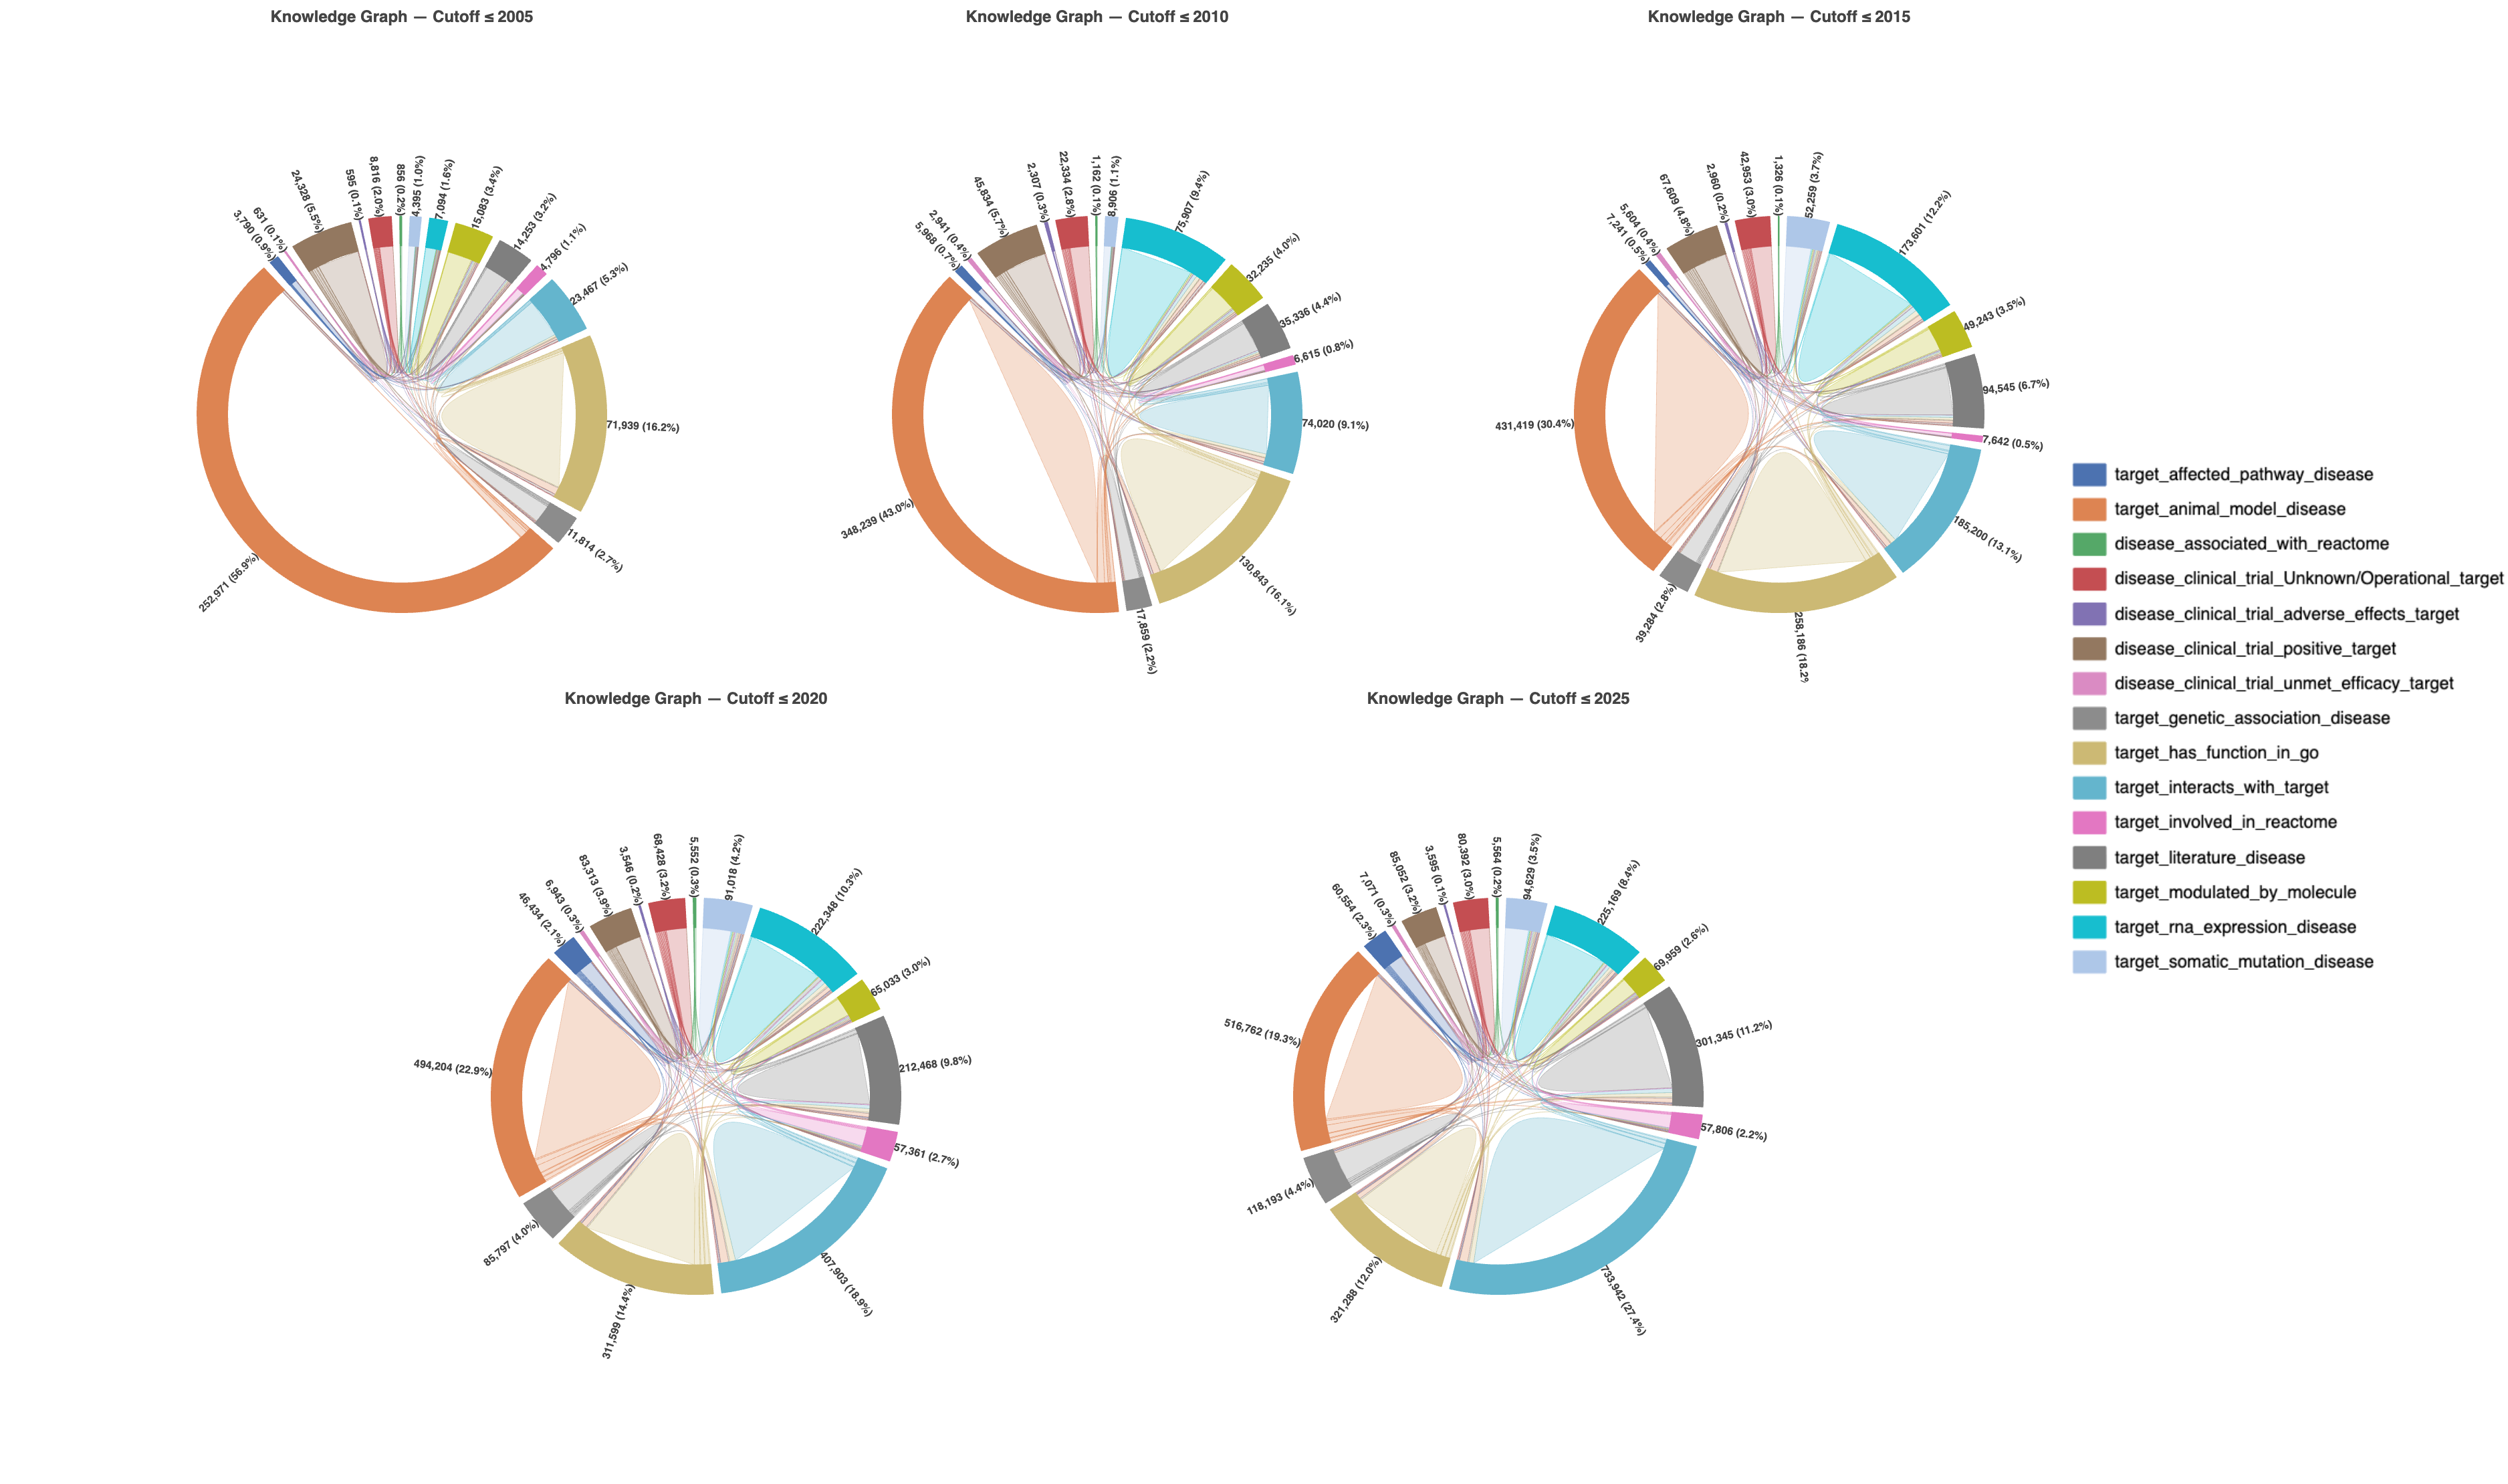
\includegraphics[width=\linewidth,height=14cm,keepaspectratio]{figures/chord_diagram.drawio.png}
\end{minipage}
\end{block}

\vspace{0.15cm}

\begin{block}{Edge-Aware Heterogeneous Graph Transformer}
{\normalsize
\begin{itemize}
  \item Extends HGT (Hu et al., 2020) with \textbf{edge feature modulation}: each edge carries $\mathbf{f}_{ts} = [s_{ts}, r_{ts}]^\top$ (cumulative + recency score), scaled by a learned $\mathbf{w}^{\phi(e)}_e \in \mathbb{R}^2$ per relation type (\textbf{+2 params only})
  \item Trained with \textbf{LambdaRank} loss optimising ranking alignment with RR@$N$
  \item 2-layer encoder ($d{=}32$) $\rightarrow$ 3-layer MLP decoder $\rightarrow$ ranking score
\end{itemize}
}
\end{block}

\end{column}

% ======== RIGHT COLUMN ========================================================
\begin{column}{.47\linewidth}

\begin{block}{Results: Relative Risk at Top-$N$}

{\normalsize 9,010 Phase~II pairs, 13 therapeutic areas, quasi-prospective split:}

\vspace{0.1cm}
\begin{tcolorbox}[colback=white, colframe=qmulblue, boxrule=1.5pt, arc=3pt,
  top=2mm, bottom=2mm]
\[
\text{RR@}N =
\frac{P(\text{advancement} \mid \text{rank} \leq N)}
     {P(\text{advancement} \mid \text{rank} > N)}
\]
\end{tcolorbox}

\vspace{0.1cm}

\begin{center}
  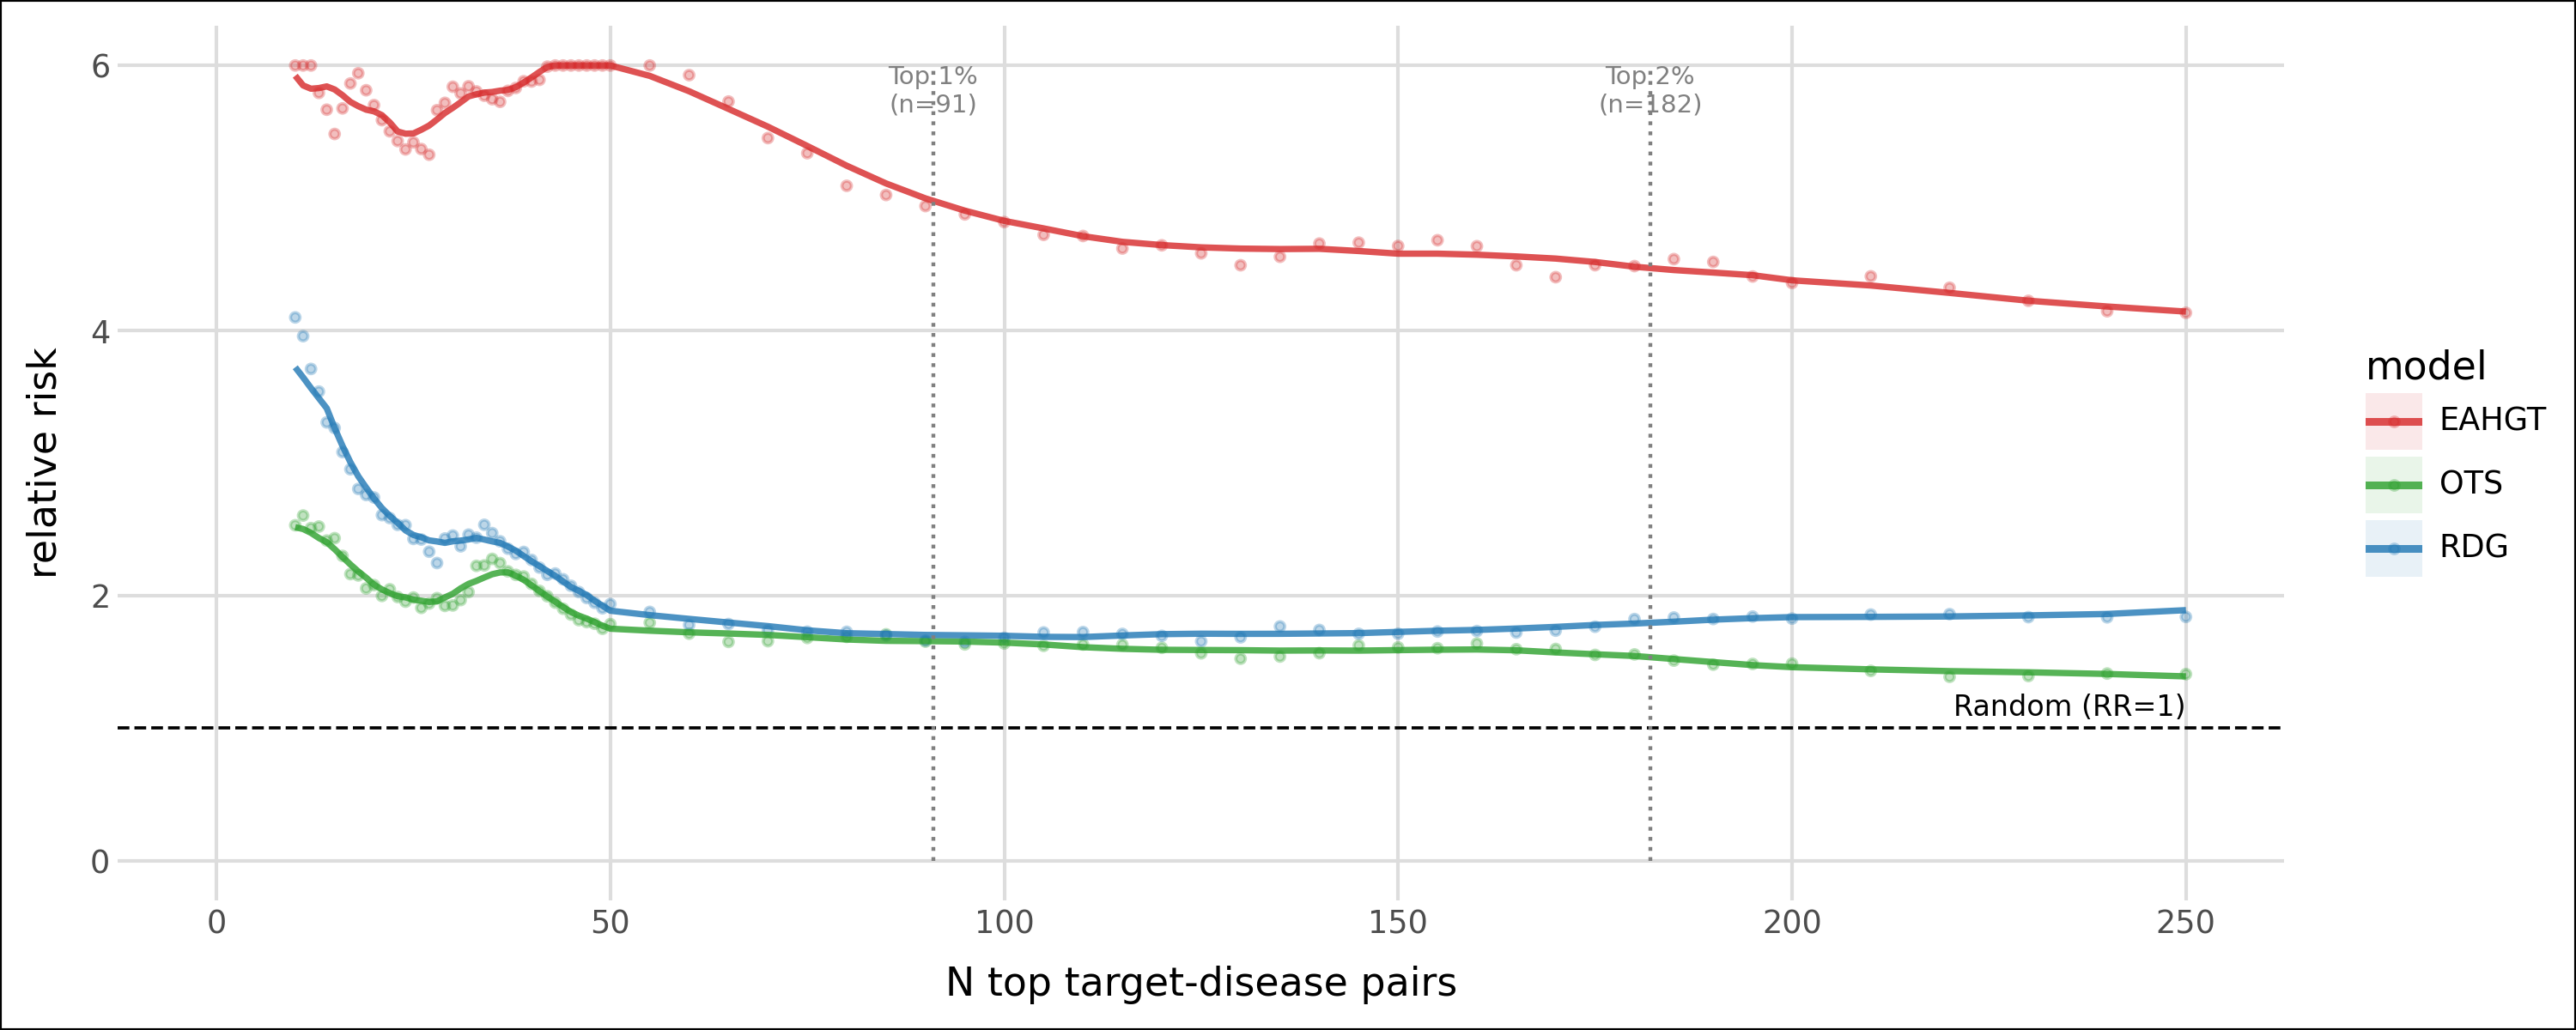
\includegraphics[width=0.85\linewidth]{figures/results/relative_risk_by_limit_katz95.png}
\end{center}

\vspace{0.1cm}

{\normalsize
\begin{itemize}
  \item \textbf{Top-10 pairs are 5.2$\times$ more likely to advance} (RR@10 = 5.23 vs.\ 4.10 for ridge baseline, \textcolor{accentgreen}{+1.13}); 95\% Katz CI entirely above baseline from $N{=}10$
\end{itemize}
}
\end{block}

\vspace{0.15cm}

\begin{block}{Results: Performance by Evidence Stratum}
\begin{center}
  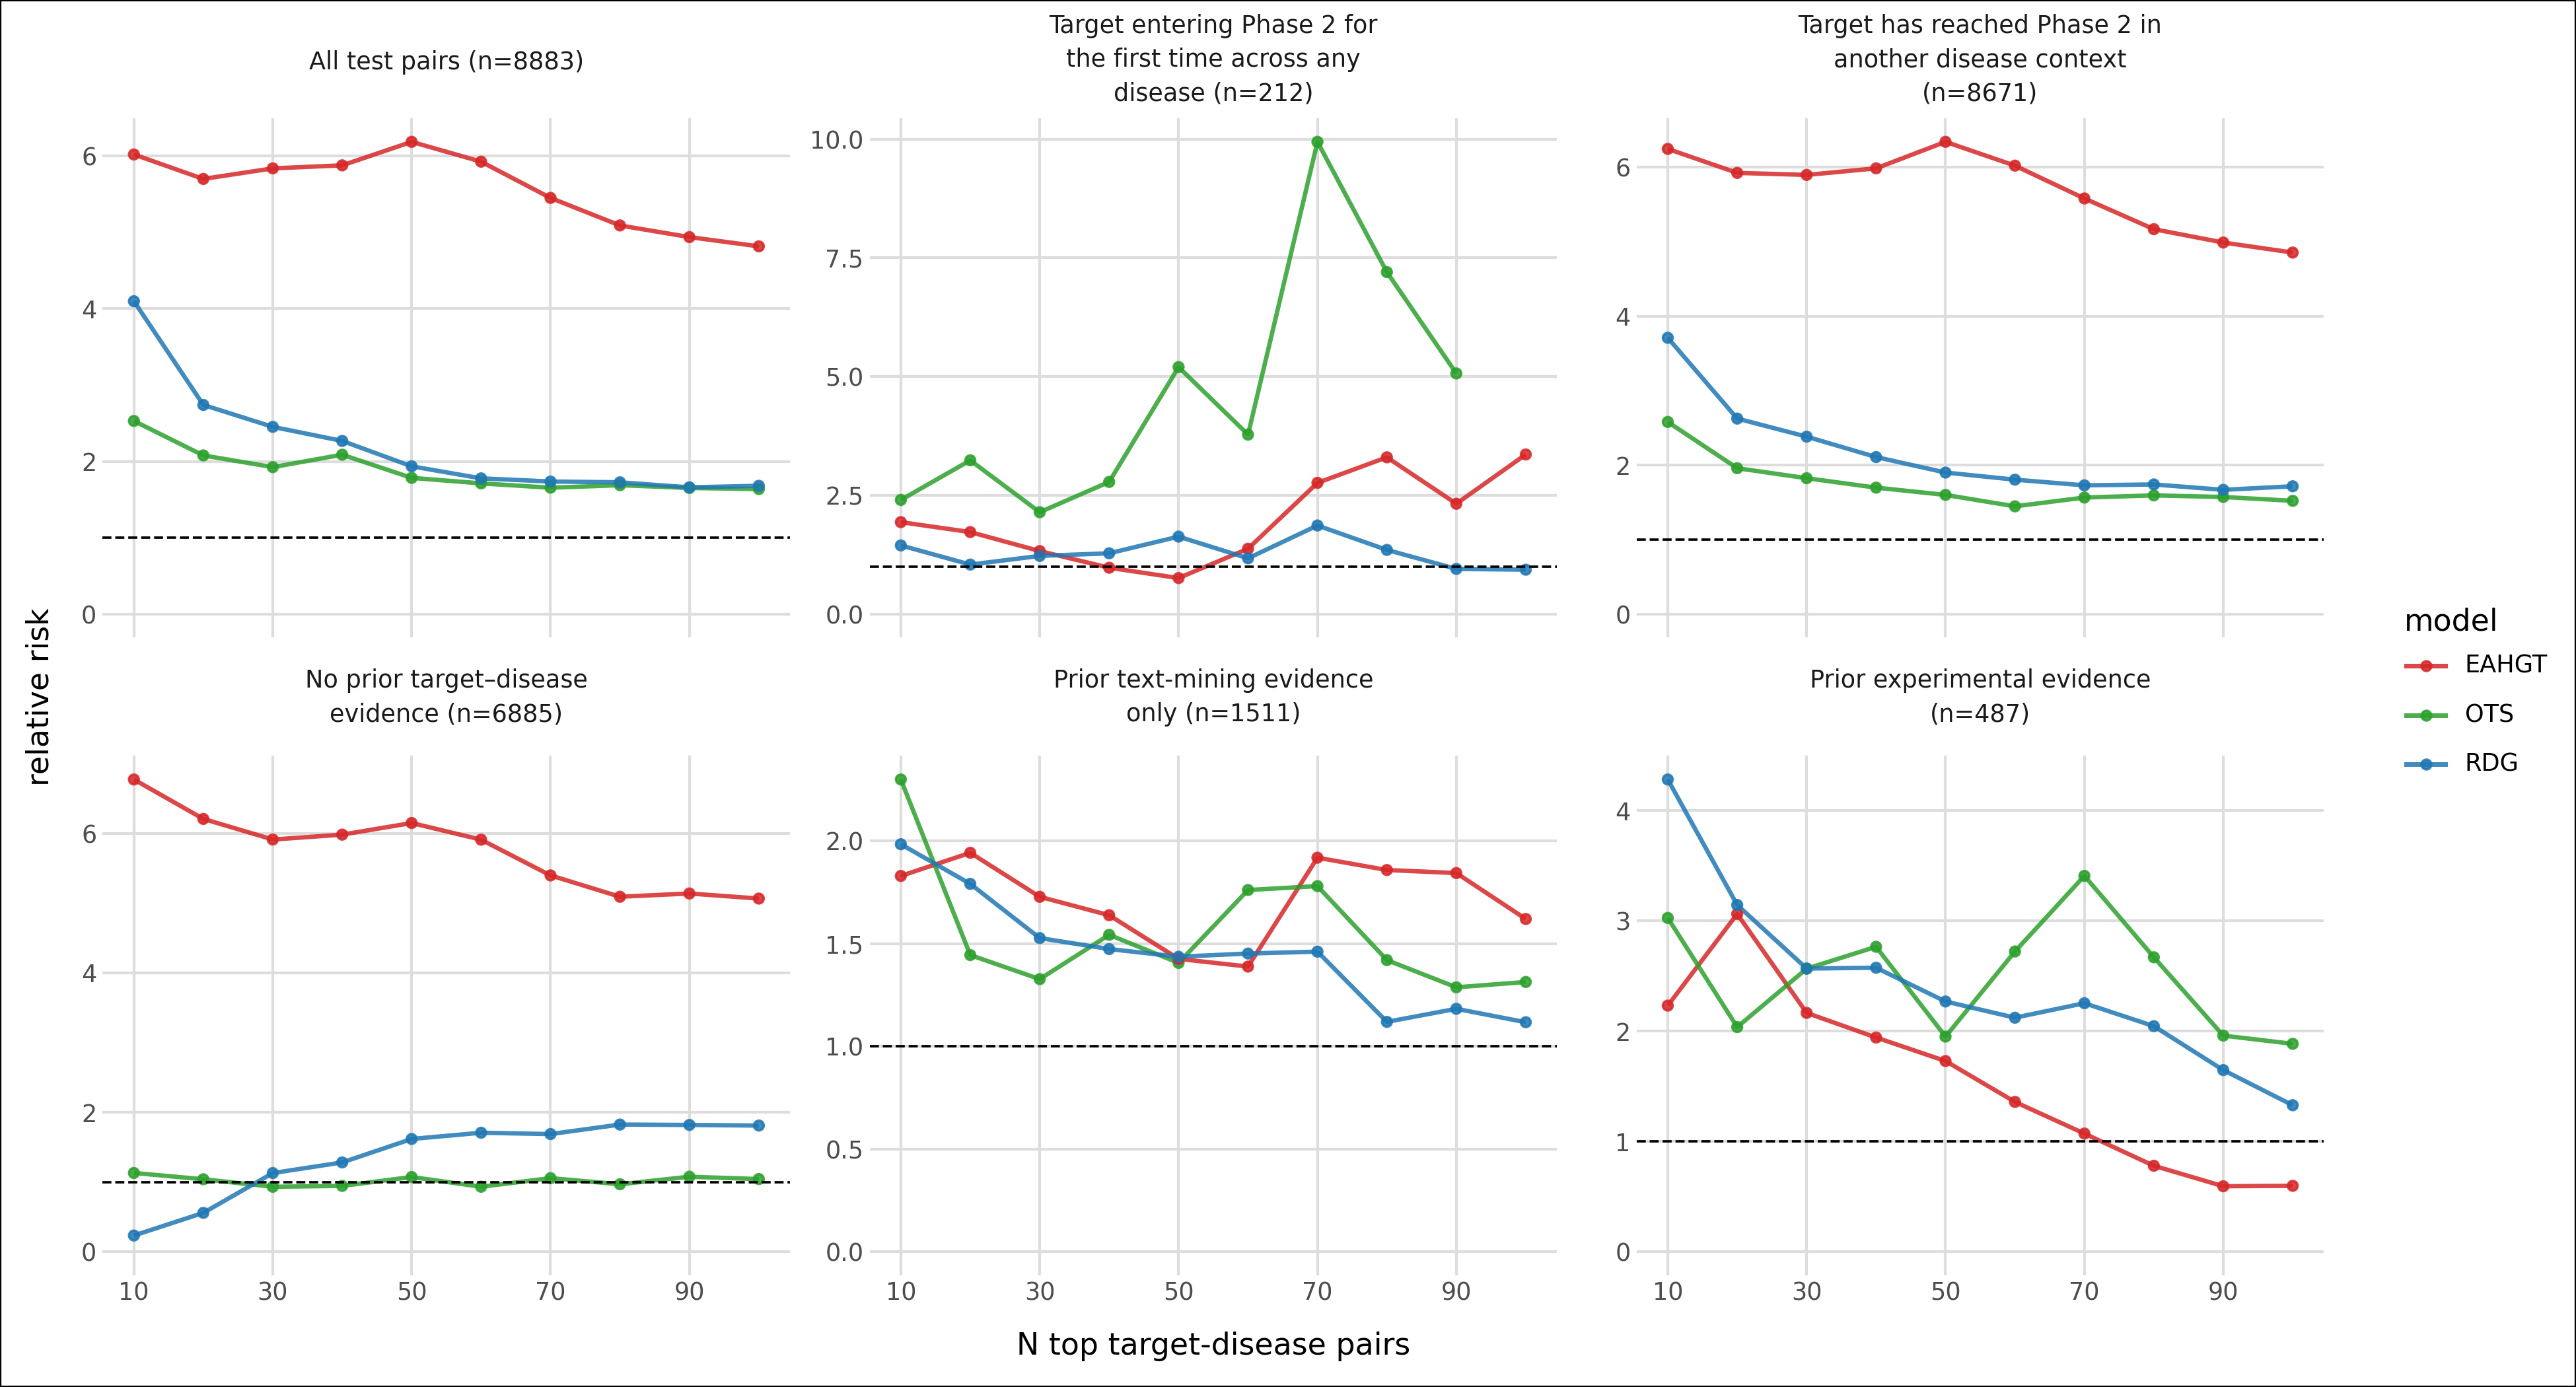
\includegraphics[width=0.85\linewidth]{figures/results/relative_risk_by_limit_by_stratum.png}
\end{center}
\vspace{0.05cm}
{\normalsize
\begin{itemize}
  \item \textbf{75\% of decisions have no direct evidence}; ridge baseline cannot rank them (RR@10 $\approx$ \textcolor{accentred}{0.22})
  \item \eahgt{} scores same pairs at \textcolor{accentgreen}{\textbf{RR@10 $\approx$ 2.64}} via indirect graph propagation and biological node feature construction
\end{itemize}
}
\end{block}

\vspace{0.15cm}

\begin{block}{Per-Therapeutic-Area Analysis}
\begin{center}
  
\includegraphics[width=0.85\linewidth]{figures/results/relative_risk_by_ta_heatmap.png}
\end{center}
\vspace{0.05cm}
{\normalsize Consistent improvement across 13 areas (Wilcoxon $p = 0.007$ at $N{=}50$). Largest gains: haematologic (+15.3), immune (+10.4), endocrine (+8.6).}
\end{block}

\vspace{0.15cm}

\begin{alertblock}{Key Contributions}
{\small
\begin{enumerate}
  \item[\textcolor{qmulblue}{\textbf{1.}}] \textbf{THBKG}: the first temporally-indexed biomedical knowledge graph with an end-to-end construction pipeline that reconstructs the evidence landscape at any historical clinical decision point, enabling quasi-prospective evaluation free from temporal inflation

  \item[\textcolor{qmulblue}{\textbf{2.}}] \textbf{Multi-hop signal recovery}: 75\% of Phase~II decisions have no direct evidence. The ridge baseline produces no usable signal (RR@10 $\approx$ 0.22); \eahgt{} recovers advancement-predictive ranking (RR@10 $\approx$ 2.64) by propagating through indirect biological paths

  \item[\textcolor{qmulblue}{\textbf{3.}}] \textbf{Portfolio de-risking}: the graph approach distinguishes programmes that are under-evidenced because curation lags behind the biology from those that genuinely lack structural support

  \item[\textcolor{qmulblue}{\textbf{4.}}] \textbf{Prospective target discovery}: target--disease pairs that score highly despite not yet having advanced through clinical trials may represent underdeveloped therapeutic opportunities where the underlying biological rationale already exists but has not yet been pursued, making them candidates for novel drug design
\end{enumerate}
}
\end{alertblock}

\end{column}
\end{columns}

\vspace{0.15cm}

% ==============================================================================
% FOOTER
% ==============================================================================
\begin{tikzpicture}[remember picture, overlay]
  % Gold accent line
  \fill[qmulgold] ([yshift=6.8cm]current page.south west) rectangle
    ([yshift=6.5cm]current page.south east);
  % Navy band
  \fill[qmulblue] ([yshift=6.5cm]current page.south west) rectangle
    (current page.south east);

  % LEFT: Logo placeholders
  % REPLACE each \node with: \node[inner sep=0] at (...) {\includegraphics[height=3cm]{logos/xxx.png}};
  \node[inner sep=0]
        at ([xshift=8cm, yshift=3.3cm]current page.south west)
        {
\includegraphics[height=2.8cm]{logos/qmul_logo_white.png}};
  \node[inner sep=0]
        at ([xshift=20cm, yshift=3.3cm]current page.south west)
        {
\includegraphics[height=2.8cm]{logos/bbsrc_ukri.png}};
  \node[inner sep=0]
        at ([xshift=30cm, yshift=3.3cm]current page.south west)
        {
\includegraphics[height=2.8cm]{logos/recursion_logo.png}};
  % RIGHT: References and contact
  \node[anchor=north east, text width=42cm, align=right, inner sep=0]
    at ([xshift=-1.5cm, yshift=6.2cm]current page.south east)

  % RIGHT: References and contact
  \node[anchor=north east, text width=42cm, align=right, inner sep=0]
    at ([xshift=-1.5cm, yshift=6.2cm]current page.south east)
    {{\color{white}\tiny
      \textbf{References:}\\[0.05cm]
      {[1]} Czech, E. et al.\ (2024) Clinical advancement forecasting. \textit{medRxiv}, 2024.08.02.24311422.\\
      {[2]} Falaguera, M.J. et al.\ (2025) Temporal trends in evidence supporting novel drug target discovery. \textit{Nat.\ Commun.}, 17, 492.\\
      {[3]} Hu, Z. et al.\ (2020) Heterogeneous Graph Transformer. \textit{WWW}, 2704--2710.\\
      {[4]} Ochoa, D. et al.\ (2021) Open Targets Platform. \textit{NAR}, 49(D1), D1302--D1310.\\
      {[5]} Wang, X. et al.\ (2018) The LambdaLoss Framework for Ranking Metric Optimization. \textit{CIKM}, ACM.\\
      {[6]} Narganes-Carlon, D. et al.\ (2024) GATher: Graph Attention Based Predictions of Gene-Disease Links. \textit{arXiv}:2409.16327.\\[0.05cm]
      \textbf{Contact:} p.siu@qmul.ac.uk
    }};
\end{tikzpicture}

\end{frame}
\end{document}